%!TEX program = pdflateX
\RequirePackage[l2tabu, orthodox]{nag}
\documentclass{book}

\usepackage[scaled=0.92]{helvet}    % set Helvetica as the sans-serif font
\renewcommand{\rmdefault}{ptm}      % set Times as the default text font
% The following loads mtpro and defines some common MTPro options [2, 4]
\usepackage[subscriptcorrection,slantedGreek,nofontinfo]{mtpro2}

\usepackage[Lenny]{fncychap}
% 9 LaTeX packages everyone should use
\usepackage{amsmath}
\usepackage[a4paper]{geometry}
\usepackage{graphicx}
\usepackage{microtype}
\usepackage{siunitx}
\usepackage{booktabs}
\usepackage[colorlinks=false, pdfborder={0 0 0}]{hyperref}
\usepackage{cleveref}



\begin{document}
\chapter{Distribution}
\section{$\Gamma$ distribution}
A random variable $X$ is said to have a $\Gamma$ distribution with parameters $\alpha,\beta$ if its probability density function is given by
\begin{equation}
    f(x;\alpha,\beta)=\frac{x^{\alpha -1}e^{-\frac{x}{\beta}}}{\beta^{\alpha}\Gamma(\alpha)},\quad \alpha,\beta\geq 0, \quad x\geq 0.
\end{equation}

The quantity $\Gamma(\alpha)$ is known as the $\Gamma$ function and it is equal to:
\begin{equation}
    \Gamma(\alpha)=\int_{0}^{\infty}x^{\alpha-1}e^{-x}\,dx
\end{equation}

$\alpha$ is \emph{shape}, $\beta$ is called \emph{scale}, and $\theta=\frac{1}{\beta}$ is called \emph{rate}.

Some useful results:
\begin{equation*}
    \mathbb{E}[X]=\alpha\beta, \quad \mathbb{V}[X]=\alpha \beta^{2},\quad \Gamma(\frac{1}{2})=\sqrt{\pi},\quad \Gamma(n)=(n-1)! .
\end{equation*}

If we set $\alpha = 1$ and $\beta=\frac{1}{\lambda}$, we get $f(x)=\lambda e^{-\lambda x}$. We see that the exponential distribution is a special case of the $\Gamma$ distribution.

\subsection{Moment Generating function}

Moment generating function of $X\sim \Gamma(\alpha,\beta)$ is
\begin{equation}
    M_{X}(t) = (1-\beta t)^{-\alpha}
\end{equation}

\noindent \textbf{Proof}:\\
\begin{equation}
    M_{X}(t)=\mathbb{E}[e^{tX}]=\int_{0}^{\infty} e^{tx}\frac{x^{\alpha-1}e^{-\frac{x}{\beta}}}{\beta^{\alpha}\Gamma(\alpha)}\,dx=\frac{1}{\beta^{\alpha}\Gamma(\alpha)}\int_{0}^{\infty} x^{\alpha-1}e^{-x(\frac{1-\beta t}{\beta})}\,dx
\end{equation}

Let $y=x\big(\frac{1-\beta t}{\beta}\big)$, then $x=\big(\frac{\beta}{1-\beta t}\big) y$, and $dx=\big(\frac{\beta}{1-\beta t}\big) dy$. Substitute these in the expression above

\begin{align}
    M_{X}(t)&=\frac{1}{\beta^{\alpha}\Gamma(\alpha)} \int_{0}^{\infty}\Big(\frac{\beta}{1-\beta t}\Big)^{\alpha-1} y^{\alpha-1}e^{-y}\frac{\beta}{1-\beta t} \,dy\\
    &= \frac{1}{\beta^{\alpha}\Gamma(\alpha)}\Big(\frac{\beta}{1-\beta t}\Big)^{\alpha}\int_{0}^{\infty} y^{\alpha-1}e^{-y}\,dy\\
    &=(1-\beta t)^{-\alpha}
\end{align}


\section{$\chi^{2}$ distribution}

Let $Z_{1},Z_{2},\ldots,Z_{k}$ be independent random variables with $Z_{i}\sim \mathcal{N}(0,1)$ (iid), then
\begin{equation}
Z=Z_{1}^{2}+Z_{2}^{2}+\cdots+Z_{k}^{2}=\sum_{i=1}^{k} Z_{i}^{2} \sim \chi^{2}_{k}
\end{equation}

 $\chi^{2}$ is a class of distribution indexed by its degree of freedom, like the $t$-distribution. In fact, $\chi^{2}$ has a relation with $t$.

If $X_1 ,X_2,\ldots,X_n$ are independent random variables with $X_{i}\sim \mathcal{N}(\mu,\sigma)$, then
\begin{equation}
X =\sum_{i=1}^{n}\bigg(\frac{X_{i}-\mu}{\sigma}\bigg)^{2}\sim \chi^{2}_{n}
\end{equation}

Let $X_{1} \sim \chi^{2}_{n}$ and $X_{2} \sim \chi^{2}_{m}$. If $X_{1}$ and $X_{2}$ are independent, then
\begin{equation}
X_{1}+X_{2} \sim \chi^{2}_{n+m}.
\end{equation}



Let $X_{1},X_{2},\ldots,X_{n}$ be independent random variables with $X_{i}\sim \mathcal{N}(\mu,\sigma)$.  Define the sample variance as
\begin{equation}
    S^{2} = \frac{1}{n-1} \sum_{i=1}^{n}(X_{i}-\bar{X})^{2}
\end{equation}
Then
\begin{equation}
    \frac{(n-1)S^{2}}{\sigma^{2}}\sim \chi^{2}_{n-1}.
\end{equation}

\subsection{shape of $\chi^{2}$ distribution}

\begin{figure}[!htbp]
\centering
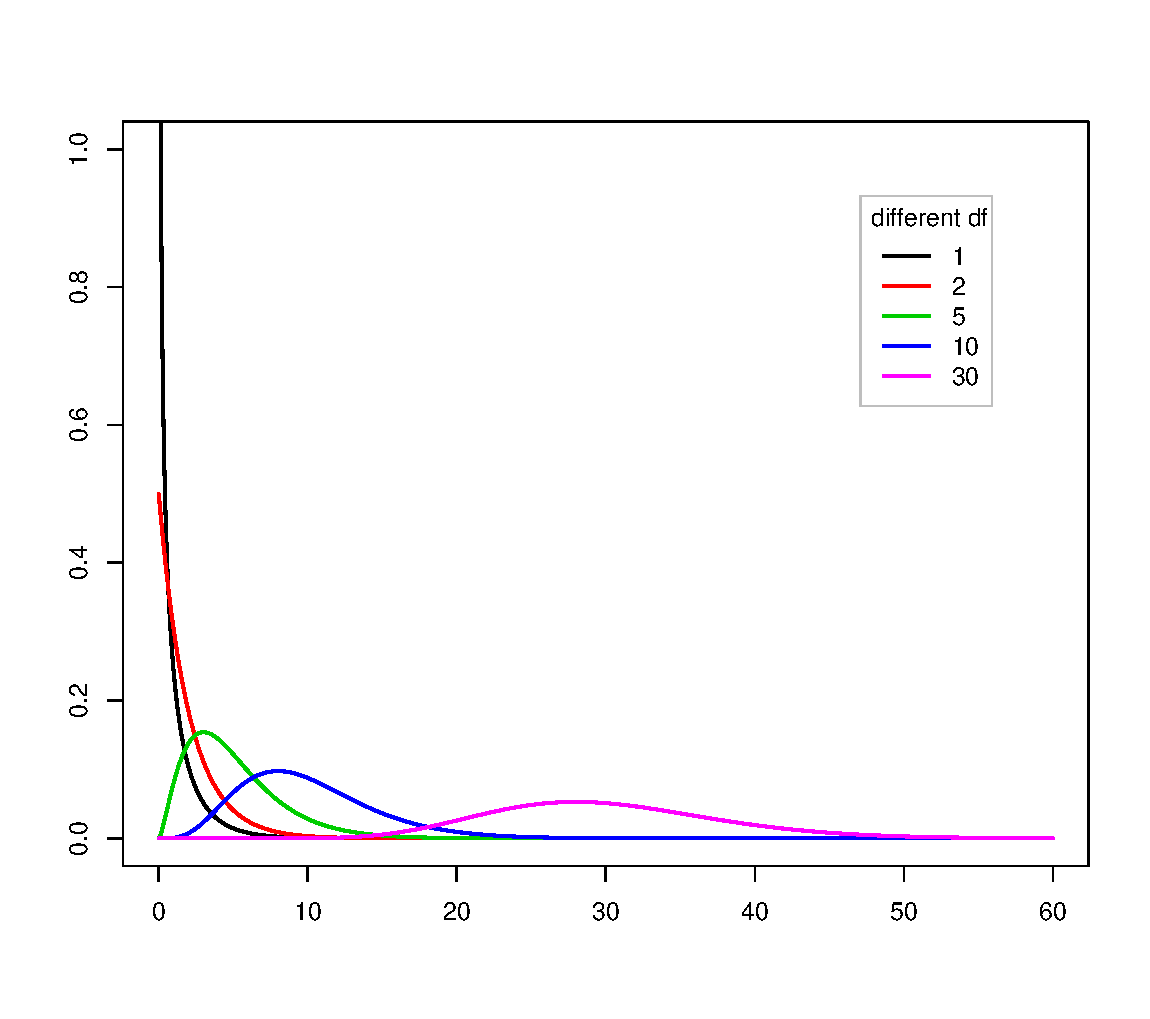
\includegraphics[width=0.6\teXtwidth]{./graph/chisq.pdf}
\caption{$\chi^{2}$ with different df}\label{fig:/graph/chisq.pdf}
\end{figure}






\end{document}
